\section{Trajectory generation}
\label{sec:trajectory_generation}


In the following, we detail the various approaches we employ for real time trajectory generation (Sec.~\ref{sub:base_motion}, \ref{sub:arm_motion}). Furthermore, we highlight the look for product (Sec.~\ref{sub:look_for_product}), pick (Sec.~\ref{sub:picking}) and place (Sec.~\ref{sub:place}) skills introduced in Fig.~\ref{fig:software_overview} and we explain how they use the trajectory generation approaches. %Finally, we cover our teaching approach (\ref{sub:teaching}), inspired by learning-from-demonstration, that provides grasping trajectories to the picking skill.

\subsection{Navigation of the base}
\label{sub:base_motion}
To navigate the mobile base in the store we employ the MoveBase navigation framework, configured with A* as the global planner and Timed-Elastic-Bands as the local planner \cite{rosmann2017integrated}.
We record a map of the environment including static obstacles prior to deployment.
Additionally, we manually define a keep-out
area to prevent the robot from going into unsafe or crowded areas, such as the checkout zones. The local planner employs the environment map and online lidar sensor information for avoiding collisions with static and moving obstacles, such as humans.

\subsection{Motion of the arm}
\label{sub:arm_motion}
To generate the motion of the arm (and base during picking), we employ the framework of \ac{fabrics}.
Fabrics is based on the composition of behaviours, defined
as differential equations in the appropriate manifolds,
which enables safe real-time planning at a very high
frequency
\cite{ratliff2023fabrics,van2022geometric,Spahn2023}. Since
\ac{fabrics} is a local, reactive trajectory generation
method, global guidance is required to perform complex
actions, such as product picking or placing. 
The global guidance for fabrics essentially consists of a sequence of local goals, where we only continue to the next goal if the previous goal has been reached. In Sec.~\ref{sub:teaching} we show how this sequence of goals, i.e., reference trajectory, can be obtained by human teaching. In the following we shortly explain how \ac{fabrics} works and how to use it.



\subsubsection{Method}
Requirements such as collision avoidance, joint-limit avoidance or self-collision avoidance are referred to in fabrics as behavioral components. Each component is represented as a differential equation of the form
$\M(\x,\xdot)\xddot+\f(\x,\xdot)=\nullvec$ on an appropriate
manifold \X{} of the configuration space \Q{}, where \M{} and \f{} are the importance metric and the forcing term respectively, and $\x$, $\xdot$ and $\xddot$ are the state, e.g., full configuration of the robot or end effector pose, and its derivatives in the manifold \X{}.
By respecting
simple construction rules, each behavioral component can be ensured to
be an optimization fabric, i.e., a dynamic system that is
stable by construction. All components can then be combined
in the robot's configuration space by applying the
operations of \textit{pull-back} and \textit{summation}. In
the configuration space, we obtain one optimization fabrics
of the form $\M\qddot + \f = \nullvec$, where $\qddot$ is the second derivative of the configuration and $\M$ and $\f$ the resulting importance metric and forcing term, respectively.
We define goal states of the robotic arm as a set of
constraints $\Sc = \{\Con_1,\Con_i,\Con_n\}$ where each
constraint \Con{} is defined by the tuple
$\Con=(\fk{p},\fk{c},\x)$. Here, $\fk{p}$ is the forward
kinematics to the parent link, $\fk{c}$ the forward
kinematics to the child link, and $\x$ is the desired position
vector. These constraints are implemented in \ac{fabrics} as a forcing term with the
differential map $\map_{\textrm{goal}} = (\fk{c} - \fk{p}) -
\x$. On the manifold defined by this differential map, we
define the forcing potential $\forc$ that can be pulled at
forcing our optimization fabric as
$\M\qddot+\f+\der{\q}{\forc} = 0$.
For further details on the definition and composition of fabrics we refer the reader to \cite{Spahn2023}.

The key advantages of \ac{fabrics} are their very fast computation and their flexibility to
compose behaviours and define the desired goal in an appropriate manifold, rather than being
fixed to defining a target configuration or end-effector pose. For
example, some tasks may require to align the end-effector
to face a point in the workspace, while
the actual position along the line is of little importance,
\cref{fig:look_for_product}.
To give another example, some products, like a can, can be grasped from many directions and one may only need to specify a subset of the desired grasping pose, e.g., the height at which the can is grasped and that the grasp should be perpendicular to the vertical axis, but not the specific direction of approach.


\begin{figure}[b]
  \centering
  \begin{subfigure}[b]{0.5\linewidth}
    \centering
    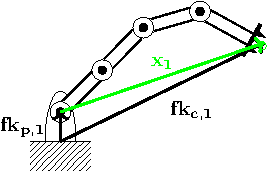
\includegraphics[width=1\textwidth]{one_constraint.pdf}
    \caption{}
    \label{subfig:one_goal_constraint}
  \end{subfigure}%
  \begin{subfigure}[b]{0.5\linewidth}
    \centering
    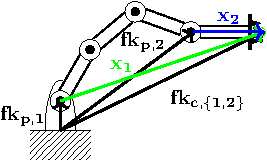
\includegraphics[width=1\textwidth]{two_constraints.pdf}
    \caption{}
    \label{subfig:two_goal_constraints}
  \end{subfigure}
  \caption{Goal constraints for \ac{fabrics}. In (a), 
  the only constraint is defined by $\Con_1 = (\fk{p,1},
  \fk{c,1}, \x_1)$.
  In (b), a second constraint is added as
   $\Con_2 = (\fk{p,2}, \fk{c,2}, \x_2)$ to align the
   end-effector horizontally.}
  \label{fig:goal_constraints}
\end{figure}

\subsubsection{Usage} As an example, a reaching problem, where the
end-effector should be at a certain position is defined by
$\Con_{\textrm{ee}} = (\fk{0},\fk{ee},\x_\textrm{ee})$,
where $\fk{0}$ is the forward kinematics to the base link of
the robot and $\x_\textrm{ee}$ the desired position of the
end-effector in the base link frame. See \cref{fig:goal_constraints} for two examples of composing goal states by constraints.

A problem we encountered when picking products with only the arm, is that the workspace of the arm is limited w.r.t. the size of the shelf. This in combination with variability in base position or product location, often resulted in the product being out of reach or requiring difficult arm configurations close to joint limits.
%As the workspace of the arm is quite limited, base navigation can be quite inaccurate, and product locations might be disturbed by other customers,
Therefore, during the picking skill, we augment arm motion by integrating the forward motion of the base as a pseudo-prismatic joint to the kinematic chain. This can be easily done in \ac{fabrics} by appending the base motion to the state vectors \q{}, \qdot{}, and \qddot{}, see \cref{fig:base_motion}. 


\subsection{Look for a product}
\label{sub:look_for_product}
Looking for the product is triggered as soon as the robotic
base is placed in front of the shelf that is expected to
have the desired product. The camera frame is then located
at a position $\x_{\camera}$. Now, the camera
must be pointed towards the expected product location, defined as
$\x_{\product}$. We can model this goal as two
constraints. First, the camera link should not move from its
current location, thus $\Con_1 =
(\fk{0},\fk{camera},\x_{\textrm{camera}})$. Secondly, the
camera should face the product location. We can compute the
ray connecting the camera and the product location
$\x_{\textrm{ray}} = \x_{\product} - \x_{\camera}$ to then
define $\Con_2 = (\fk{7}, \fk{8},  \x_{\textrm{ray}})$
that effectively aligns the end-effector with the previously
defined ray $\x_{\textrm{ray}}$, see
\cref{fig:look_for_product}.

\begin{figure}
  \begin{center}
    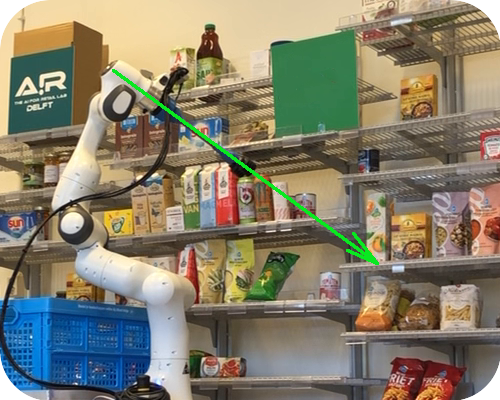
\includegraphics[width=0.55\linewidth]{look_for_item_wo.png}
  \end{center}
  \caption{Illustration of the orientation constraints for trajectory
  generation for the look-for-product skill.}
  \label{fig:look_for_product}
\end{figure}


\subsection{Picking of a product}
\label{sub:picking}
To define a goal for picking products we use a combination of three constraints.
First, the position of the vacuum cup is determined by the
position of the product, thus $\Con_1 =
(\fk{0},\fk{suction-cup}, \x_{\textrm{suction}}, \weight_{\textrm{suction}})$. Secondly, we
limit  ourselves to picking products from the shelf, thus
constraining the end-effector to be perpendicular to the
shelf by defining $\Con_2 = (\fk{7},\fk{8}, \x_{7,8})$. Lastly, our gripper is composed of two
suction cups, which, depending on the product should align with a specific angle for executing the most reliable grasp. The desired alignment defines
our third constraint for the picking as $\Con_3 =
(\fk{suction1}, \fk{suction2}, \x_{\textrm{alignment}})$. Although it is possible to
program a picking action, including approach and retreat, as a sequence of this set of
constraints, it is difficult to capture all the nuances of
picking in the code. Therefore, we make use of a human operator to teach the robot the best trajectory to reliably pick specific products, following the 
learning-from-demonstration paradigm
\cite{celemin2022interactive}. Teaching has proven an effective way to generate sequences of the previously mentioned
constraints thus encoding the human understanding of the picking problem into recorded trajectories. We explain the process of
recording and playing back trajectories in detail in Sec.~\ref{sub:teaching}. 
%

%

\subsection{Placing of a product}
\label{sub:place}

Placing the product consists of four phases. The robot navigates
to a configuration to its right or to its left depending on
whether it was a right-sided pick or a left-sided pick.
Then, it moves above the crate facing downwards. This is
defined by two constraints, $\Con_1 = (\fk{0},\fk{8},
\x_{0,8}, 1)$ and $\Con_2 = (\fk{7},\fk{8}, \x_{7,8})$.
The product is then placed by moving the arm downwards until an
external force, from touching the bottom of the crate
or an already placed product, is detected. That triggers the
release of the gripper and changes the goal to the homing
position ready for the next product.
% In
% case, the robot is commanded with a goal defined in the
% configuration space, we limit motion to the arm. All other
% goals are composed as a union of \textit{goal-constraints}.
% A goal-constraint is a defined by a desired distance vector
% between two links on the kinematic chain. 








